\chapter{Methodology}
\label{cha:5}

\section{Pre-processing}

\subsection{Dataset split}

The dataset reliability scores are grouped and split into 4 classes based on its reliability score as previously described in Section \ref{bat-characteristics}:
\begin{enumerate}
    \item Problematic ---> scores between 0.00 and 24.00
    \item Questionable ---> scores between 24.01 and 32.00
    \item Generally Reliable ---> scores between 32.01 and 40.00
    \item Reliable ---> scores between 40.01 and 64
\end{enumerate}

The dataset is then split into three sets of train, test, and validation with the following distribution:
\begin{itemize}
    \item Train set: 4325 rows \\
          287 samples of class 'Problematic', 611 samples of class 'Questionable', 1033 samples of class 'Generally Reliable', 2394 of class 'Reliable'
    \item Test set: 569 rows \\
          27 samples of class 'Problematic', 54 samples of class 'Questionable', 104 samples of class 'Generally Reliable', 384 of class 'Reliable'
    \item Validation set: 603 rows \\
          34 samples of class 'Problematic', 70 samples of class 'Questionable', 128 samples of class 'Generally Reliable', 371 of class 'Reliable'
\end{itemize}

The split is done in a way to ensure that articles from different outlets are distributed equally between the three sets. This is done by first grouping the articles based on their outlet and labels, then iterating over each group, splitting the rows equally, and distributing to the train, test, and validation set. Groups of less than 5 rows that are not enough to be split and therefore appended to the train set. To handle class imbalances, weighted loss is used when training the model, with weights in proportion to the distribution of each class.

A major drawback of this 'balance' splitting is that there is no unseen outlet in the test set and validation set. This can influence the final test metrics and may hinder the model's ability to generalise to new, unseen articles from unseen outlets. However, considering that new outlets are rarely introduced in the real life, it might be beneficial to slightly overfit on the patterns of existing outlets.


\section{Features and baselines}

The primary features will include the title and content of the articles. Ideally, a reliable article-level bias classifier should be able to generalise solely or mainly from the content of the articles, capturing the context of the article will be the key element of reliable performance. However, outlet information is also experimented and compared.

As baselines, traditional encoding methods such as Bag-of-Words and TF-IDF are implemented, combined with a simple logistic regression as a classifier. In these cases, the validation set are concatenated into the training set. An outlet majority votes is also implemented as a comparison to show the influence of outlet information in this particular task. This method works by simply taking the majority vote over classes for every outlet and use it as a classifier: \textit{an article is from outlet A, majority of articles from outlet A is classified as class X, therefore, article A has a class X}.

\section{Proposed methods}

\subsection{BoW + MLP}

\begin{figure}[htbp]
    \centering
    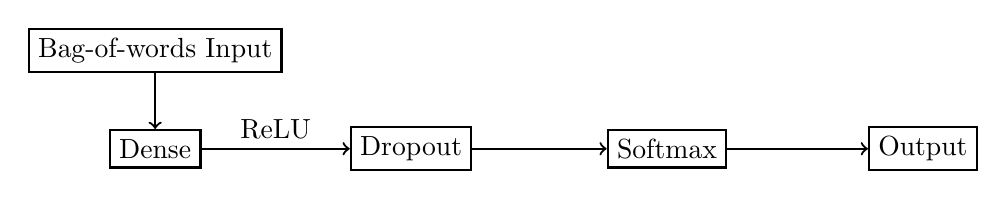
\begin{tikzpicture}[
            node distance=1.25cm,
            every node/.style={fill=white, font=\footnotesize},
            thick, scale=1, every node/.style={scale=1}]

        \node (input) [draw, align=center] {Bag-of-words Input};
        \node (dense) [draw, below of=input] {Dense};
        \draw[->] (input.south) -- (dense.north);
        \node (dropout) [draw, right of=dense, xshift=2cm] {Dropout};
        \draw[->] (dense.east) -- node[above, midway] {ReLU} (dropout.west);
        \node (softmax) [draw, right of=dropout, xshift=2cm] {Softmax};
        \draw[->] (dropout.east) -- (softmax.west);
        \node (output) [draw, right of=softmax, xshift=2cm] {Output};
        \draw[->] (softmax.east) -- (output.west);

    \end{tikzpicture}
    \caption{BoW + MLP architecture. The input article is encoded as a bag of words, then feed into a single linear multilayer perceptron before softmax operation.}
    \label{fig:bow_mlp_architecture}
\end{figure}

Figure \ref{fig:bow_mlp_architecture} shows the simple diagram of the BoW + MLP method, combining traditional encoding methods with a simple neural network training. This approach allows for a simple and computationally-cheap implementation, yet effective classifier. The model is trained on 10 epochs with a learning rate of 2e-5. Hidden size for the dense layer is 128 with a dropout probability of 0.2, no warmup steps are applied.

\subsection{BERT fine-tuning}

\begin{figure}[htbp]
    \centering
    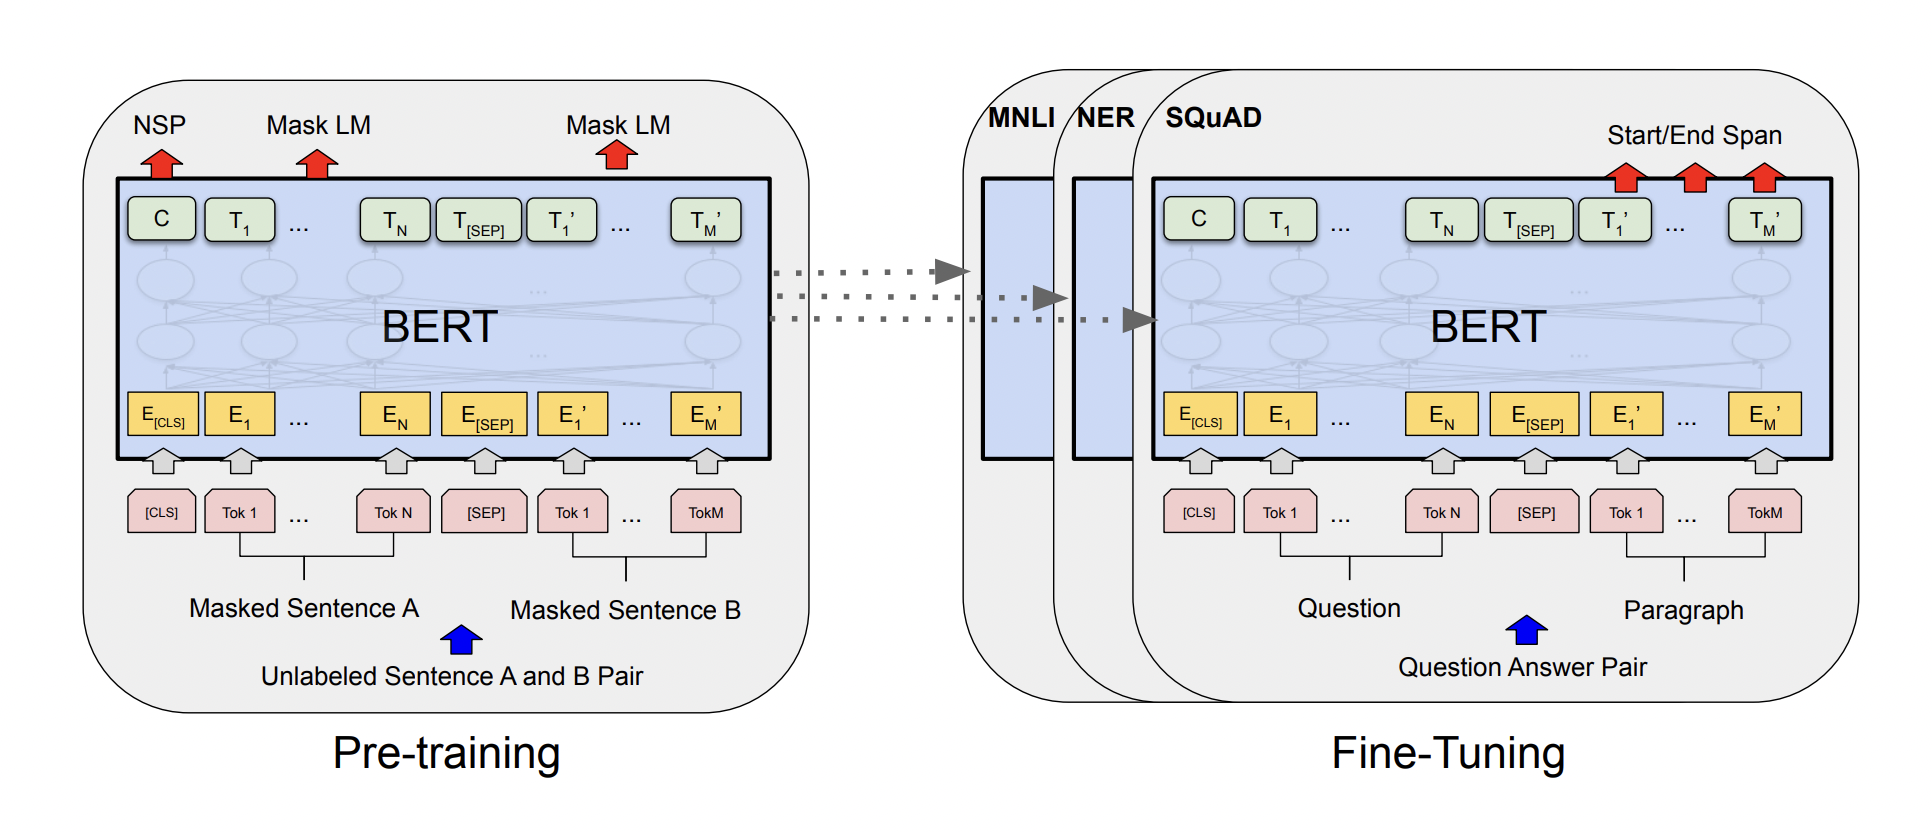
\includegraphics[width=0.9\linewidth]{images/bert_finetuning.png}
    \caption{BERT pre-training and fine-tuning procedures \cite{devlin-2019-bert}}
    \label{fig:bert_finetuning}
\end{figure}

A fine-tuning operation is done as described in the original BERT paper \cite{devlin-2019-bert}, where input texts are tokenised and fed into a pre-trained BERT model for a downstream task. This approach leverages the powerful pre-trained representations from BERT and adapts them to the specific requirements of the downstream task with relatively small amounts of task-specific training data. This method has become a widely common and popular technique for performing various NLP tasks due to its effectiveness in improving performance over traditional models.

Fine-tuning is done over 4 epochs with weighted loss, 2e-5 learning rate, and 500 linear warmup steps.

\subsection{BERT sliding window fine-tuning}

\begin{figure}[htbp]
    \centering
    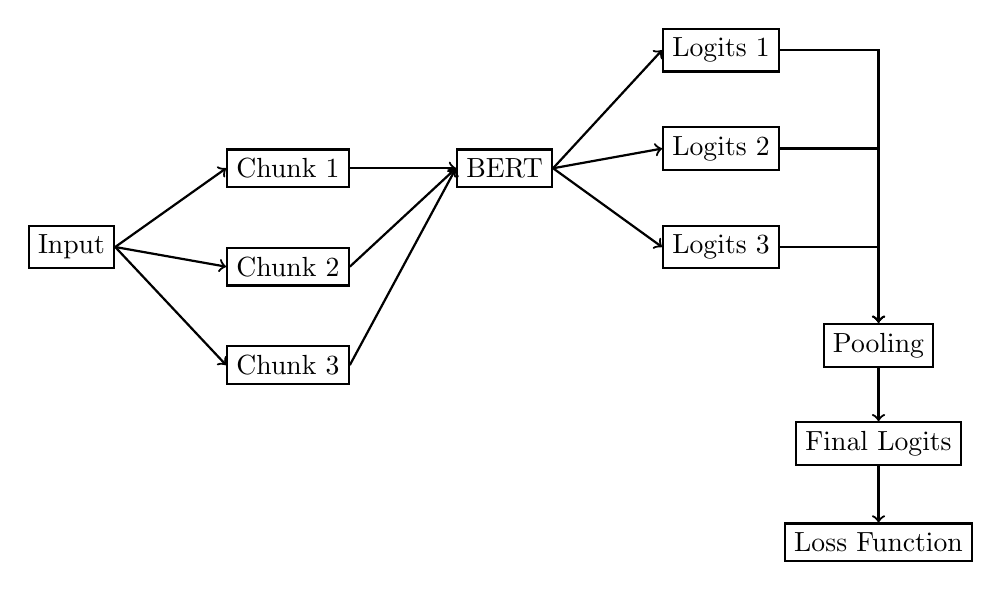
\begin{tikzpicture}[
            node distance=1.25cm,
            every node/.style={fill=white, font=\footnotesize},
            thick, scale=1, every node/.style={scale=1}
        ]

        \node (input) [draw, align=center] {Input};

        \node (chunk1) [draw, right of=input, xshift=1.5cm, yshift=1cm] {Chunk 1};
        \node (chunk2) [draw, below of=chunk1] {Chunk 2};
        \node (chunk3) [draw, below of=chunk2] {Chunk 3};

        \draw[->] (input.east) -- (chunk1.west);
        \draw[->] (input.east) -- (chunk2.west);
        \draw[->] (input.east) -- (chunk3.west);

        \node (bert) [draw, right of=chunk1, xshift=1.5cm] {BERT};

        \draw[->] (chunk1.east) -- (bert.west);
        \draw[->] (chunk2.east) -- (bert.west);
        \draw[->] (chunk3.east) -- (bert.west);

        \node (logits1) [draw, right of=bert, xshift=1.5cm, yshift=1.5cm] {Logits 1};
        \node (logits2) [draw, below of=logits1] {Logits 2};
        \node (logits3) [draw, below of=logits2] {Logits 3};

        \draw[->] (bert.east) -- (logits1.west);
        \draw[->] (bert.east) -- (logits2.west);
        \draw[->] (bert.east) -- (logits3.west);

        \node (pooling) [draw, below of=logits3, xshift=2cm, align=center] {Pooling};

        \draw[->] (logits1.east) -- ++(0.5cm,0) -| (pooling.north);
        \draw[->] (logits2.east) -- ++(0.5cm,0) -| (pooling.north);
        \draw[->] (logits3.east) -- ++(0.5cm,0) -| (pooling.north);

        \node (final_logits) [draw, below of=pooling] {Final Logits};

        \draw[->] (pooling.south) -- (final_logits.north);

        \node (loss) [draw, below of=final_logits] {Loss Function};

        \draw[->] (final_logits.south) -- (loss.north);
    \end{tikzpicture}
    \caption{BERT Sliding window fine-tuning architecture. The input article is split into chunks, each chunk is processed by the model as a mini batch, and the resulting logits are pooled before applying the loss function.}
    \label{fig:sliding_window_architecture}
\end{figure}

Figure \ref{fig:sliding_window_architecture} illustrates the architecture of the sliding window fine-tuning method. Input texts are segmented into chunks, which are then processed as mini-batches by the model. The logits (output scores) produced by each chunk are then pooled together to produce the final logits, to which the loss function is applied. This method bypasses the sequence length limitation of BERT models (512 tokens), allowing for full representation and processing of text input without any loss of information.

A window size of 512 is chosen in the implementation with no stride. Similarly, fine-tuning is done over 4 epochs with weighted loss, 2e-5 learning rate, and 500 linear warmup steps.

\begin{comment}
The complexity of this method is as follows:
\[
    O(L \cdot T \cdot H)
\]

where L is the sequence length, T is the number of Transformer layers in the BERT model (typically 12), H is Hidden size of the BERT model (dimension of the Transformer's feedforward networks, typically 768).
\end{comment}

\subsection{CLS method}


\begin{figure}[htbp]
    \centering

    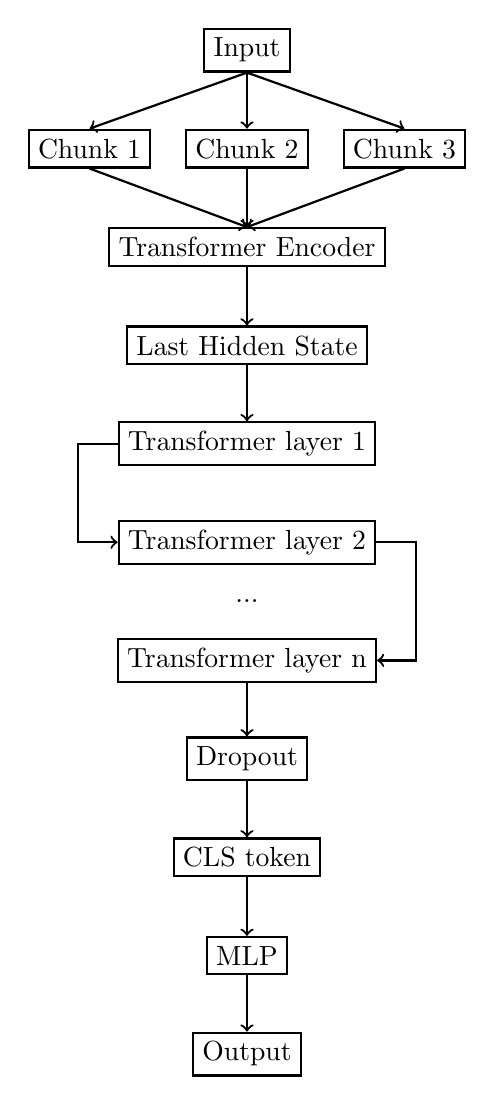
\begin{tikzpicture}[
            node distance=1.25cm,
            every node/.style={fill=white, font=\footnotesize},
            thick, scale=1, every node/.style={scale=1}]


        \node (input) [draw, align=center] {Input};

        \node (chunk1) [draw, below of=input, xshift=-2cm] {Chunk 1};
        \node (chunk2) [draw, below of=input] {Chunk 2};
        \node (chunk3) [draw, below of=input, xshift=2cm] {Chunk 3};

        \draw[->] (input.south) -- (chunk1.north);
        \draw[->] (input.south) -- (chunk2.north);
        \draw[->] (input.south) -- (chunk3.north);

        \node (encoder) [draw, below of=chunk2] {Transformer Encoder};

        \draw[->] (chunk1.south) -- (encoder.north);
        \draw[->] (chunk2.south) -- (encoder.north);
        \draw[->] (chunk3.south) -- (encoder.north);

        \node(hidden) [draw, below of=encoder] {Last Hidden State};

        \draw[->] (encoder.south) -- (hidden.north);

        \node (transformer1) [draw, below of=hidden] {Transformer layer 1};
        \node (transformer2) [draw, below of=transformer1] {Transformer layer 2};
        \node (transformern) [draw, below of=transformer2, yshift=-0.25cm] {Transformer layer n};
        \node (transformer_dots) [below of=transformer2, node distance=0.75cm] {...};

        \draw[->] (hidden.south) -- (transformer1.north);
        \draw[->] (transformer1.west) -- ++(-0.5cm,0) |- (transformer2.west);
        \draw[->] (transformer2.east) -- ++(0.5cm,0) |- (transformern.east);

        \node (dropout) [draw, below of=transformern] {Dropout};

        \draw[->] (transformern.south) -- (dropout.north);

        \node (cls) [draw, rectangle, below of=dropout] {CLS token};

        \draw[->] (dropout.south) -- (cls.north);

        \node (mlp) [draw, rectangle, below of=cls] {MLP};

        \draw[->] (cls.south) -- (mlp.north);

        \node (output) [draw, rectangle, below of=mlp] {Output};

        \draw[->] (mlp.south) -- (output.north);


    \end{tikzpicture}
    \caption{CLS method architecture}
    \label{fig:cls_method}
\end{figure}

Figure \ref{fig:cls_method} shows the full architecture of the CLS method. This method begins by similarly segmenting the input text into smaller chunks. These chunks are encoded into a higher dimensional space features by feeding them into a pre-trained Large Language Model (LLM) and extracting the last hidden state, also known as \textit{feature-based approach} as described in \cite{sun-2020-fine-tune}. Subsequently, the chunks are then passed into \textit{n} Transformer layers to enrich their contextual understanding. For each chunk, only the representation of the CLS token (the first token) is retained (CLS Pooling, as in \cite{su-2021-classifying}), serving as a concise summary of the entire chunk sequence. This summary representation is then processed through a Multi-Layer Perceptron (MLP). Finally, a softmax operation will be applied to the output of the MLP layer to determine the final output class. Using a LLM as an encoder and taking its last hidden state allows for a good contextual representation of each chunk. By only using the CLS token representation instead of the whole chunk, this method allows for a more effective, yet simpler approach compared to other chunk pooling methods.

Two different language models can be used as the Transformer encoder in this method: BERT \cite{devlin-2019-bert} or MAGPIE \cite{horych-2024-magpie}. The MLP consists of two linear layers with ReLu activation function \cite{agarap-2018-relu} and dropouts. Each chunk is set to contain 512 tokens, only 2 Transformer layers are used, and 0.2 probability is applied to the dropout layer. Training is done over 3 epochs with weighted loss, 1e-5 learning rate and 162 warmup steps (10\% of total training steps).

\begin{comment}
The complexity of the CLS method can be expressed as:
\[
    O(L \cdot TF \cdot T \cdot H_{\text{enc}}^2 \cdot M \cdot H_{\text{mlp}}^2)
\]

where:
\begin{align*}
    L              & : \text{Sequence length (number of tokens)}, \\
    T              & : \text{Number of Transformer layers},       \\
    H_{\text{enc}} & : \text{Hidden size of Transformer layers},  \\
    M              & : \text{Number of layers in the MLP},        \\
    H_{\text{mlp}} & : \text{Hidden size of the MLP}.             \\
\end{align*}
\end{comment}

\section{Training details}

All methods are implemented in Python 3.12.0 \cite{van-1995-python} using the PyTorch \cite{paszke-2017-pytorch} and Transformer \cite{wolf-2020-huggingface} package from HuggingFace. The BERT model utilised in these methods is the 'bert-base-cased' instead of the 'bert-base-uncased' to account for distinctions in capitalised words, which may be crucial \cite{devlin-2019-bert}. AdamW \cite{loshchilov-2019-adamw} optimiser and Cross Entropy Loss is used in all cases.

\subsection{Weighted loss}

Weighted loss addresses the problem of training models on an imbalanced dataset by assigning higher weights to classes with fewer instances and lower weights to classes with more instances. This adjustment ensures that the model pays more attention to correctly predicting the minority class, thereby improving overall performance metrics. Using weighted loss during training is preferred over oversampling the minority class. Oversampling can introduce abstract examples that may not accurately represent real-world articles, potentially leading to less effective model performance.

Weighted loss is calculated through the scikit-learn library \cite{pedregosa-2011-scikit-learn} and inserted into the loss function. Figure \ref{fig:class_weight} shows the calculated class weight for each class in the training set.


\begin{figure}[htbp]
    \centering
    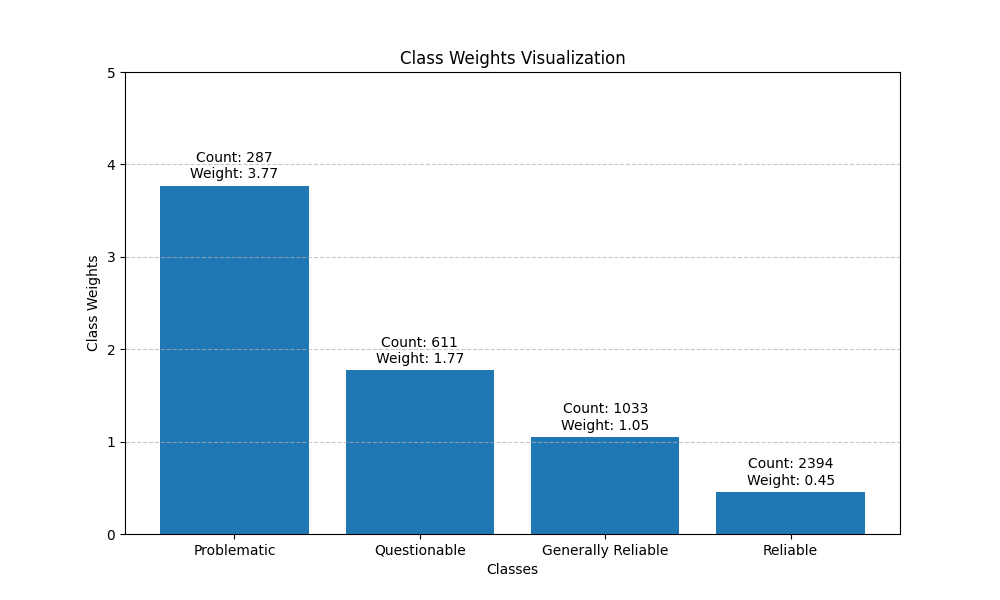
\includegraphics[width=0.9\linewidth]{figures/class_weight.png}
    \caption{Class weight in the training set}
    \label{fig:class_weight}
\end{figure}



%%% Local Variables: 
%%% mode: latex
%%% TeX-master: "thesis"
%%% End: 
